\documentclass[english,serif,mathserif,xcolor=pdftex,dvipsnames,table]{beamer}
\usepackage{gc3}

\newcommand{\vcenteredinclude}[2]{\begingroup
\setbox0=\hbox{\includegraphics[width=#1cm]{#2}}%
\parbox{\wd0}{\box0}\endgroup}

\title[Cloud@UZH]{%
  Hobbes: \\
  the University of Zurich's \\ 
  IaaS cloud
}
\author[Sergio Maffioletti]{%
  Sergio Maffioletti \\
  S3IT: Service and Support for ScienceIT, \\
  University of Zurich
}
\date{June.18, 2014}

\begin{document}

% title frame
\maketitle

\begin{frame}
\begin{center}
\large{why is the University of Zurich \\
      investing in IaaS ?}
\end{center}
\end{frame}

\begin{frame}
  \frametitle{Today's computational research needs}
  Requirements from research groups are variegated. \\
  They need more and more {\color{Blue}integrated services} and not a
  collection of {\color{Blue}individual} infrastructure.

  \begin{itemize}
  \item A computational cluster is {\color{Blue}only one} of the
    services that needs to be provided.
  \item Need of {\color{Blue}specialized} resources
  \item Need to integrate {\color{Blue}local storage}
  \item Need to access {\color{Blue}Windows} based resources
  \item Need to attach computational and storage resources to specific
    {\color{Blue}instrument}
  \end{itemize}
\end{frame}


\begin{frame}
  \frametitle{Let's have few examples of what we have to deal with}
  
  \begin{itemize}
  \item {\color{Blue}Dedicated processing server}: users creates their
    own customized processing services for their specific data
    analysis. (like a {\color{Blue}supersized} version of their
    {\color{Blue}workstation})
  \item {\color{Blue}Customized environments}: users can deploy and
    configure their own applications and all sort of tools they might
    require (e.g. mysql database).
  \item {\color{Blue}Community tools}: users wish to reuse tools
    tailored for their research but developed for specific platforms
    (e.g. Hadoop, Shark, etc.).
  \end{itemize}
\end{frame}

\begin{frame}
  \frametitle{Let's have few examples of what we have to deal with}
  
  \begin{itemize}
  \item {\color{Blue}Interactive Windows}: some image processing tools
    are only available in Windows and require interactive access.
  \item {\color{Blue}Reuse existing pipelines}: users wish to re-use
    existing pipelines written for a specific batch-system (e.g. SGE,
    condor) or a specific type of resource (e.g. CentOS 5.3).
  \item {\color{Blue}Scale from application level}: run Matlab mDCE
    or parallel R or iPython cluster. 
  \end{itemize}
\end{frame}

\begin{frame}
  \frametitle{the Research Infrastructure provider point of view}

  \begin{itemize}
  \item Accommodate all of these needs (and there are much more) is
    {\color{Blue}complicated}.
  \item I wish they could all be supported with a {\color{Blue}single
      infrastructure}.
  \end{itemize}
\end{frame}

\begin{frame}
  \frametitle{the UZH IaaS Hobbes}

\url{http://www.s3it.uzh.ch/infrastructure/hobbes}

\+
{\color{Blue}OpenStack}-based IaaS solution, specifically
      targeted to address large scale computational research.

      \+
The main {\color{Blue}research infrastructure instrument}
      available for the whole university.

  % \begin{itemize}
  %   \item \url{http://www.s3it.uzh.ch/infrastructure/hobbes}
  %   \item {\color{Blue}OpenStack}-based IaaS solution, specifically
  %     targeted to address large scale computational research.
  %   \item The main {\color{Blue}research infrastructure instrument}
  %     available for the whole university.
  % \end{itemize}
 \end{frame}

\begin{frame}
  \frametitle{Cloud @ UZH}

  \begin{tabular}{lp{7cm}}
    {\color{Blue}October 2012} & first prototype installation \\
    {\color{Blue}March 2013} & testbed open to academic users
    (codename: {\color{Blue}Hobbes}) \\
  {\color{Blue}Mar-Dec 2013} & used as
    {\color{Blue}High-Throughput} data analysis system\\
    & \scriptsize{
    \begin{itemize}
      \item {\color{Blue}94 users} (on average 70\% active)
      \item {\color{Blue}40 different} research groups (30 internal 10
    external) 
  \end{itemize}} \\
  {\color{Blue}October 2013} &Increased capacity (860 cores
  and 3.2TB RAM)\\
  {\color{Blue}January 2014} &Enter production stage\\
  \end{tabular}
\end{frame}

\begin{frame}[fragile]
  \frametitle{Hardware specs}
  
  Veeery heterogeneous hardware\dots
  
  \small{
    \begin{center}
      \begin{tabular}{llll}
        Q.ty	& Model	& CPU	& RAM \\
        17x	& Dell PE1955	& 2x Quad-core	& 8GB \\
        12x	& Dell M605	& 2x Quad-core 	& 16GB \\
        10x	& Dell M600	& 2x Quad-core 	& 16GB \\
        12x	& Dalco Servers	& 2x Quad-Core 	& 32GB \\
        14x	& Dell M620	& 2x Eight-core & 128GB \\
        1x	& SGI UV100	& 8x Six-core 	& 512GB \\
      \end{tabular}
    \end{center}
  }
\end{frame}

\begin{frame}
  \frametitle{Hobbes helps us provide user support}
  
  \begin{block}{Application level integration}
    \begin{itemize}
    \item Matlab mDCE supported through {\color{Blue}automated tools}:
      \href{http://gc3-uzh-ch.github.io/elasticluster/}{elasticluster}
    \item Easily accommodate {\color{Blue}existing workloads}.
    \item No longer need {\color{Blue}batch-processing} system if not
      required:
      \href{https://code.google.com/p/gc3pie/}{gc3pie}
    \item Provide support at {\color{Blue}application integration}
      level.
    \end{itemize}
  \end{block}
\end{frame}

\begin{frame}
  \frametitle{Hobbes helps us provide user support}
  
  \begin{block}{Build support infrastructure}
    \begin{itemize}
    \item {\color{Blue}Dedicated processing server}: User can create
      their own instances, attach their own volumes and
      run their own processing service.
    \item {\color{Blue}Customized environments and Community tools}:
      Users can evaluate all sort of platforms and/or
      existing community solutions.
    \item Possibility of accessing {\color{Blue}commercial providers}
    \item Possibility of supporting usecases {\color{Blue}already
        running} on commercial providers.
    \end{itemize}
  \end{block}
\end{frame}

\begin{frame}
  \frametitle{What next}

  \begin{itemize}
    \item {\color{Blue}Fall 2014}: Public procurement published for
      further expand Hobbes
    \item {\color{Blue}Q1 2015}: Integrate existing Hobbes with
      purchased system and re-purposed nodes from Schroedinger
    \item This should lead to a {\color{Blue}100TFlop} cloud system.
    % \item Expected size: {\color{Blue}4'500} compute cores and
    %   {\color{Blue}16TB} of aggregated memory.
    \item \url{http://www.s3it.uzh.ch/infrastructure/hobbes}.
  \end{itemize}
\begin{center}
Thank you for your attention!
\end{center}
\end{frame}

\begin{frame}
  \frametitle{Software specs}

  \small{
    \vcenteredinclude{2}{fig/openstack.jpg} (Folsom) IaaS cloud
    infrastructure \\
    \vcenteredinclude{2}{fig/cfengine.png} deployment and configuration
    manager \\
    \vcenteredinclude{2}{fig/ubuntu.jpg} 12.04 as base system
  }
\end{frame}

\begin{frame}
  \frametitle{OpenStack logical view}
  
  \begin{tikzpicture}
    \node (0,0){
      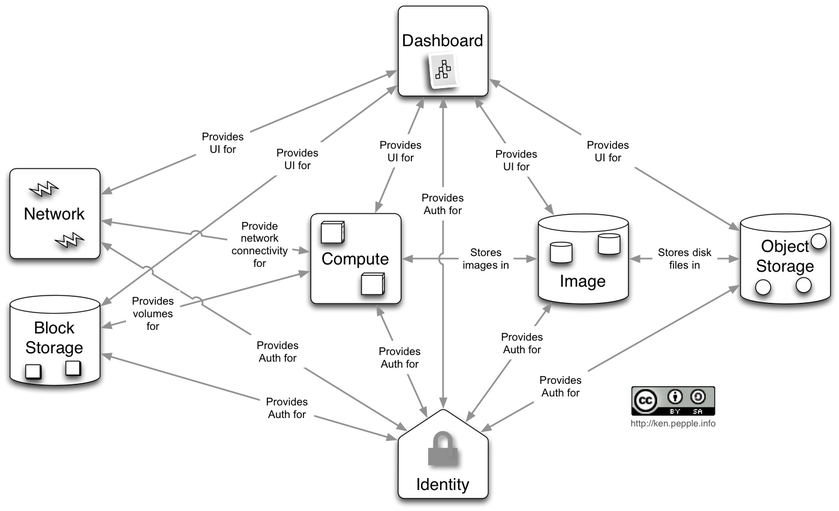
\includegraphics[width=\linewidth]{fig/openstack-conceptual-arch.png}};
    % identity
    \visible<2>{\draw[red, fill=red, opacity=0.3] (0.25,-2.5) circle (0.9);}
    % compute
    \visible<3>{\draw[red, fill=red, opacity=0.3] (-0.8,-0.05) circle (0.9);}
    % neutron
    \visible<4>{\draw[red, fill=red, opacity=0.3] (-4.5,0.5) circle (0.9);}
    % image
    \visible<5>{\draw[red, fill=red, opacity=0.3] (2,-0.05) circle (0.9);}
    % block
    \visible<6>{\draw[red, fill=red, opacity=0.3] (-4.5,-1.1) circle (0.9);}
    % object
    \visible<7>{\draw[red, fill=red, opacity=0.3] (4.48,-0.05) circle (0.9);}
    % dashboard
    \visible<8>{\draw[red, fill=red, opacity=0.3] (0.3,2.5) circle (0.9);}
  \end{tikzpicture}

  \alt<1>{\vspace{1.4em}}{~}
  \alt<2>{\textbf{Keystone} provides the authentication service}{}
  \alt<3>{\textbf{Nova} provides computational services}{}
  \alt<4>{\textbf{Neutron} provides network services}{}
  \alt<5>{\textbf{Glance} provides image store}{}
  \alt<6>{\textbf{Cinder} provides block persistent store}{}
  \alt<7>{\textbf{Swift} provides object persistent store}{}
  \alt<8>{\textbf{Horizon} provides web user interface}{}
\end{frame}


\end{document}
